\section{Results}
\label{sec:results}

\subsection{Read-out: a chat-generator direction (H1)}
\label{sec:readout}

\begin{figure}[t]
    \centering
    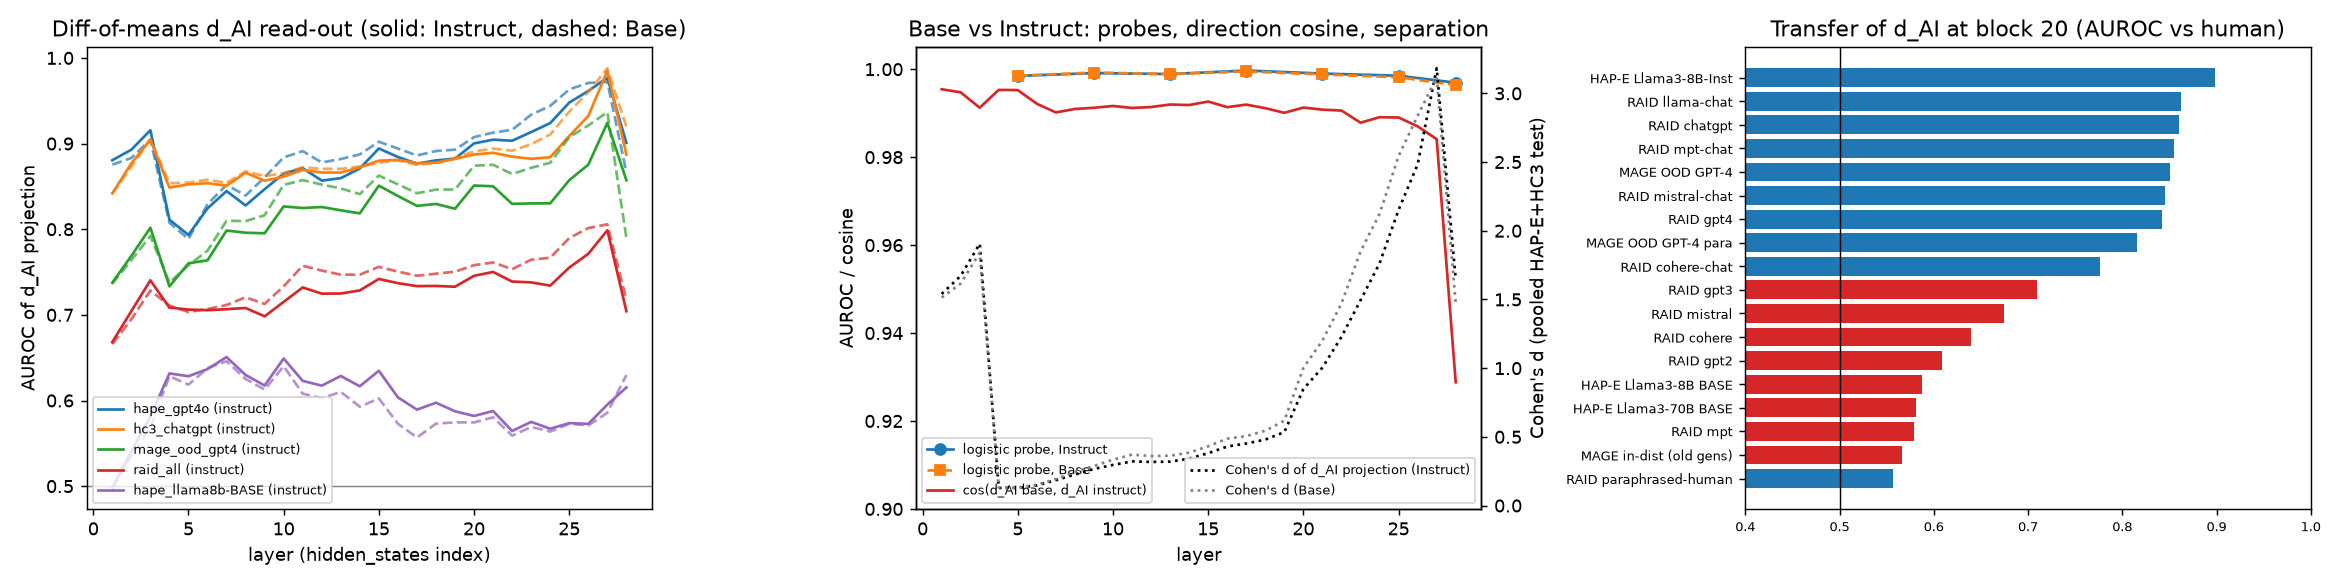
\includegraphics[width=0.99\linewidth]{figures/readout_layers_transfer.png}
    \caption{Read-out of \dai. \figleft{} AUROC of the \dai projection per layer for the instruct (solid) and base (dashed) models. Separation is good for chat generators but near chance for Llama-3-8B {\em base} continuations (purple). \figcenter{} Logistic probes reach 0.999 in both models, and $\cos(\daibase,\daiinst)$ stays $\ge 0.98$ at every layer. \figright{} Transfer at block 20: \dai separates chat and instruct generators (blue) from human text, but barely separates base and older LMs (red).}
    \label{fig:readout}
\end{figure}

\begin{table}[t]
    \centering
    \small
    \begin{tabular}{@{}lcc@{}}
        \toprule
        Test set (AUROC of \dai projection, block 20) & \textsc{Instruct} & \textsc{Base} \\
        \midrule
        \hape GPT-4o \versus human (same prefix) & 0.905 & {\bf 0.913} \\
        \hape Llama-3-8B-Instruct (unseen generator) & 0.899 & {\bf 0.909} \\
        \hcthree ChatGPT \versus human (same question) & 0.889 & {\bf 0.894} \\
        Fit \hape $\to$ test \hcthree / fit \hcthree $\to$ test \hape & 0.88 / 0.85 & 0.89 / 0.87 \\
        \mage OOD GPT-4 / GPT-4-paraphrased & 0.85 / 0.82 & 0.88 / 0.85 \\
        \raid chat generators (5) & 0.84--0.86 & 0.85--0.87 \\
        \midrule
        \raid base / older LMs (5) & 0.58--0.71 & 0.59--0.72 \\
        \hape Llama-3-8B / 70B {\em base} continuations & 0.59 / 0.58 & 0.58 / 0.58 \\
        \mage in-distribution (older generators) & 0.57 & 0.58 \\
        \raid paraphrased human \versus human & 0.56 & 0.55 \\
        \midrule
        Logistic probe, matched test (blocks 4--27) & 0.997--0.9997 & 0.996--0.9995 \\
        10 random directions (\hcthree, block 14) & 0.27--0.67 & -- \\
        \bottomrule
    \end{tabular}
    \caption{Read-out and transfer of \dai. A single direction separates content-matched pairs (AUROC $\approx$ 0.89--0.91) and transfers to unseen chat generators, but not to text from base LMs (bottom block). The base model's direction reads out equally well or slightly better.}
    \label{tab:readout}
\end{table}


{\bf Does a single direction separate human from AI text?} Yes. At block 20, the \dai projection reaches AUROC 0.89--0.91 on held-out content-matched pairs (\tabref{tab:readout}). It transfers across datasets (fitting on \hape and testing on \hcthree gives 0.88), to an unseen instruct generator (0.899), and to \raid and \mage chat generators (0.82--0.86).
It fails, however, on text from {\em base} language models: 0.58 on Llama-3 base continuations and 0.58--0.71 on older \raid generators (\figref{fig:readout}, right). A full logistic probe is near-perfect (0.997--0.9997), replicating \citet{quaremba2026linear}, but it uses many directions. We steer with the one-dimensional \dai because it is a cleaner object.
Random directions alone reach AUROCs between 0.27 and 0.67, because the residual stream is anisotropic, so moderate AUROCs ($\le 0.7$) for any single direction carry little meaning.

\subsection{Disentanglement: not formality, not the Assistant (H3)}
\label{sec:disentangle}

\begin{table}[t]
    \centering
    \small
    \begin{tabular}{@{}lccc@{}}
        \toprule
        Direction (block 20) & Raw cos with \dai & Whitened cos & AUROC (matched test) \\
        \midrule
        \dai & 1 & 1 & 0.869 \\
        \daiperp (6 confounds removed) & 0.78 & 0.26 & {\bf 0.970} \\
        \midrule
        Formality & $-0.23$ & 0.02 & 0.32 (0.68 flipped) \\
        Fluency (log-prob) & 0.06 & 0.05 & 0.51 \\
        Word length & 0.55 & $-0.01$ & 0.69 \\
        Domain (Reddit) & $-0.02$ & 0.01 & 0.51 \\
        Verbosity & 0.28 & 0.01 & 0.69 \\
        Assistant axis & 0.25 & {\bf 0.005} & 0.54 \\
        Post-training (Llama inst $-$ base) & {\bf 0.90} & 0.20 & 0.88 \\
        \midrule
        Null: random human/human split & $-0.09$ & 0.008 & 0.39 \\
        \bottomrule
    \end{tabular}
    \caption{Overlap of \dai with confound directions. In whitened geometry \dai is nearly orthogonal to every confound ($|\cos|\le 0.05$). The one large raw overlap is with an instruct-minus-base direction from Llama-3.}
    \label{tab:disentangle}
\end{table}


\Tabref{tab:disentangle} compares \dai with the confound directions. Raw cosines are misleading: word length (0.55), verbosity (0.28), and the Assistant axis (0.25) look related, but even a random split of human texts has raw cosine 0.44 with formality. After whitening, \dai is nearly orthogonal to every confound ($|\cos| \le 0.05$), including the Assistant axis (0.005).
Projecting the six-confound subspace out and refitting {\em raises} the difference-of-means AUROC from 0.89 to 0.98; the confounds added noise, not signal.
A cross-validated logistic regression on nine text covariates plus domain dummies reaches AUROC 0.944. The covariates are formality, log-probability, word length, length, contractions, an AI-ism lexicon, distinct-2, first person, and markdown. Adding the \dai projection raises this to 0.956. So \dai carries information beyond surface statistics, though it correlates moderately with some of them ($|r|\le 0.38$: longer words, fewer contractions, less first person).

{\bf What is \dai, then?} The one large overlap is with the {\em post-training} direction: Llama-3 instruct minus base continuations of the same prefix, from a different model family (raw cosine 0.90, whitened 0.20). Together with the transfer pattern in \secref{sec:readout}, this suggests that \dai encodes the style that instruction tuning produces, not ``machine-generated'' text in general.

\subsection{Causal steering (H2)}
\label{sec:steer}

\begin{figure}[t]
    \centering
    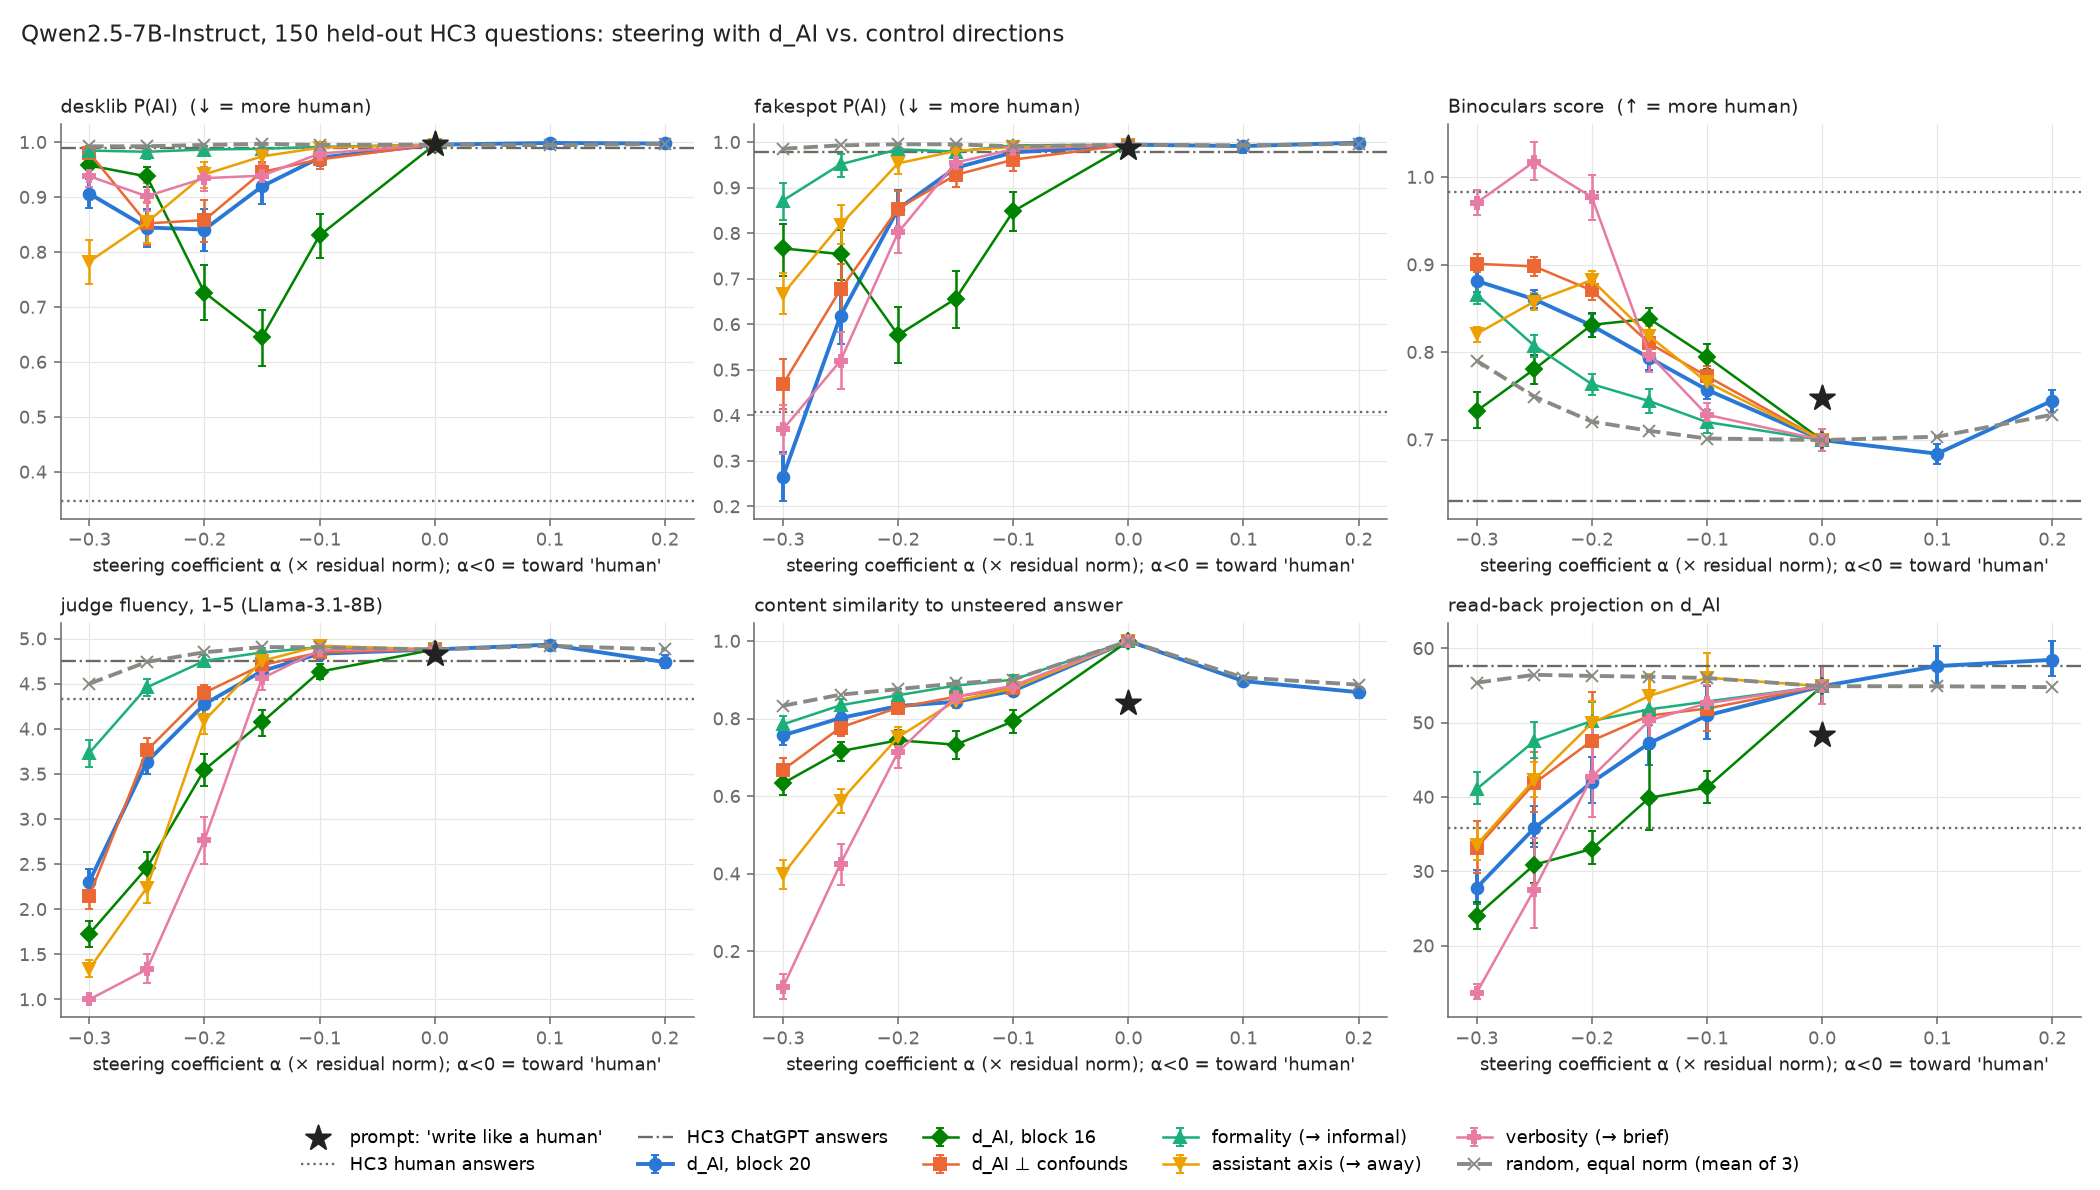
\includegraphics[width=0.99\linewidth]{figures/fig1_steer_dose_response.png}
    \caption{Dose--response of steering \qwen (150 held-out questions, 95\% CIs). {\em Top:} \dai at block 20 (blue), \daiperp (orange), and \dai at block 16 (dark green) lower the supervised detectors, while equal-norm random directions (gray) stay at ceiling. \binoculars rises for every perturbation, random included. {\em Bottom:} the cost in fluency, content similarity, and read-back projection. The ``write like a human'' prompt (star) leaves the supervised detectors untouched. Dotted and dash-dotted lines are \hcthree human and ChatGPT references.}
    \label{fig:dose}
\end{figure}

\begin{table}[t]
    \centering
    \resizebox{\textwidth}{!}{%
    \begin{tabular}{@{}lccccccc@{}}
        \toprule
        & \multicolumn{3}{c}{AI-ness} & \multicolumn{3}{c}{Coherence and content} & \\
        \cmidrule(lr){2-4} \cmidrule(lr){5-7}
        Condition & \desklib $\downarrow$ & \fakespot $\downarrow$ & \binoculars $\uparrow$ & Fluency & Relevance & Sim.\ to unsteered & Read-back \\
        \midrule
        Unsteered & 0.996 & 0.994 & 0.700 & 4.88 & 4.89 & 1.00 & 54.9 \\
        \midrule
        \dai $\alpha=-0.1$ & 0.972 & 0.978 & 0.757 & 4.83 & 4.89 & 0.87 & 51.0 \\
        \dai $\alpha=-0.15$ & 0.920 & 0.944 & 0.793 & 4.64 & 4.85 & 0.84 & 47.2 \\
        \dai $\alpha=-0.2$ & {\bf 0.841} & 0.853 & 0.830 & 4.27 & 4.72 & 0.83 & 42.0 \\
        \dai $\alpha=-0.25$ & 0.845 & 0.619 & 0.860 & 3.63 & 4.10 & 0.80 & 35.8 \\
        \dai $\alpha=-0.3$ & 0.906 & {\bf 0.266} & {\bf 0.881} & 2.31 & 2.52 & 0.76 & 27.8 \\
        \dai $\alpha=+0.2$ & 0.998 & 0.999 & 0.745 & 4.74 & 4.62 & 0.87 & 58.4 \\
        \daiperp $\alpha=-0.2$ & 0.858 & 0.854 & 0.871 & 4.40 & 4.61 & 0.83 & 47.6 \\
        Block-16 \dai $\alpha=-0.15$ & {\bf 0.645} & 0.656 & 0.838 & 4.07 & 4.33 & 0.73 & 39.9 \\
        \midrule
        Random (mean of 3) $\alpha=-0.2$ & 0.995 & 0.996 & 0.721 & 4.85 & 4.80 & 0.88 & 56.3 \\
        Random (mean of 3) $\alpha=-0.3$ & 0.993 & 0.986 & 0.790 & 4.50 & 4.53 & 0.83 & 55.4 \\
        Formality $\alpha=-0.25$ & 0.983 & 0.952 & 0.807 & 4.46 & 4.66 & 0.83 & 47.5 \\
        Formality $\alpha=-0.3$ & 0.985 & 0.872 & 0.866 & 3.73 & 4.00 & 0.79 & 41.1 \\
        Assistant axis $\alpha=-0.2$ & 0.941 & 0.954 & 0.882 & 4.09 & 3.57 & 0.75 & 49.9 \\
        Assistant axis $\alpha=-0.3$ & 0.783 & 0.667 & 0.821 & 1.34 & 1.02 & 0.40 & 33.6 \\
        Verbosity $\alpha=-0.15$ & 0.939 & 0.955 & 0.797 & 4.56 & 4.71 & 0.86 & 50.3 \\
        Prompt ``write like a human'' & 0.996 & 0.988 & 0.747 & 4.83 & 4.89 & 0.84 & 48.4 \\
        Prompt + \dai $\alpha=-0.15$ & 0.835 & 0.899 & 0.851 & 4.11 & 4.73 & 0.76 & 32.8 \\
        Zero-ablation of \dai (blocks 10--27) & 0.967 & 0.317 & 0.861 & 1.00 & 1.00 & 0.03 & 74.8 \\
        \midrule
        {\em \hcthree human answers} & {\em 0.348} & {\em 0.408} & {\em 0.982} & {\em 4.33} & {\em 4.26} & -- & {\em 35.8} \\
        {\em \hcthree ChatGPT answers} & {\em 0.990} & {\em 0.978} & {\em 0.630} & {\em 4.75} & {\em 4.83} & -- & {\em 57.6} \\
        \bottomrule
    \end{tabular}
    }
    \caption{Steering \qwen at block 20 (unless noted), means over 150 held-out questions. Negative $\alpha$ moves toward ``human''. Fluency and relevance are 1--5 judge scores (Llama-3.1-8B). Read-back is the unsteered model's projection of the output onto \dai. Best AI-ness values among steered conditions in {\bf bold}; note that the strongest values come with degraded fluency, so \figref{fig:matched} compares methods at matched coherence.}
    \label{tab:steer_main}
\end{table}


{\bf Does subtracting \dai make output read as more human?} Yes, on all three valid detectors. At block 20 and $\alpha=-0.2$, \desklib \pai falls from 0.996 to 0.841, \fakespot from 0.994 to 0.853, and \binoculars rises from 0.70 to 0.83 (\tabref{tab:steer_main}, \figref{fig:dose}).
Random directions of equal norm leave the supervised detectors at 0.99. Paired per prompt against the mean of three random directions, \dai lowers \desklib by $-0.154$ [$-0.20$, $-0.11$] ($p<10^{-10}$) and raises \binoculars by $+0.109$ at $\alpha=-0.2$. At $\alpha=-0.15$ the gaps are $-0.077$ and $+0.083$ (all $p<10^{-3}$).
The cost is a fluency drop from 4.88 to 4.27 at $\alpha=-0.2$ (\versus 4.85 for random). Relevance stays at 4.72, and similarity to the unsteered answer is 0.83 (\versus 0.88).
\daiperp, with all six confounds projected out, steers as well as \dai ($\desklib=0.858$ at $\alpha=-0.2$).
The ``write like a human'' prompt does not move \desklib at all (0.996).

\begin{figure}[t]
    \centering
    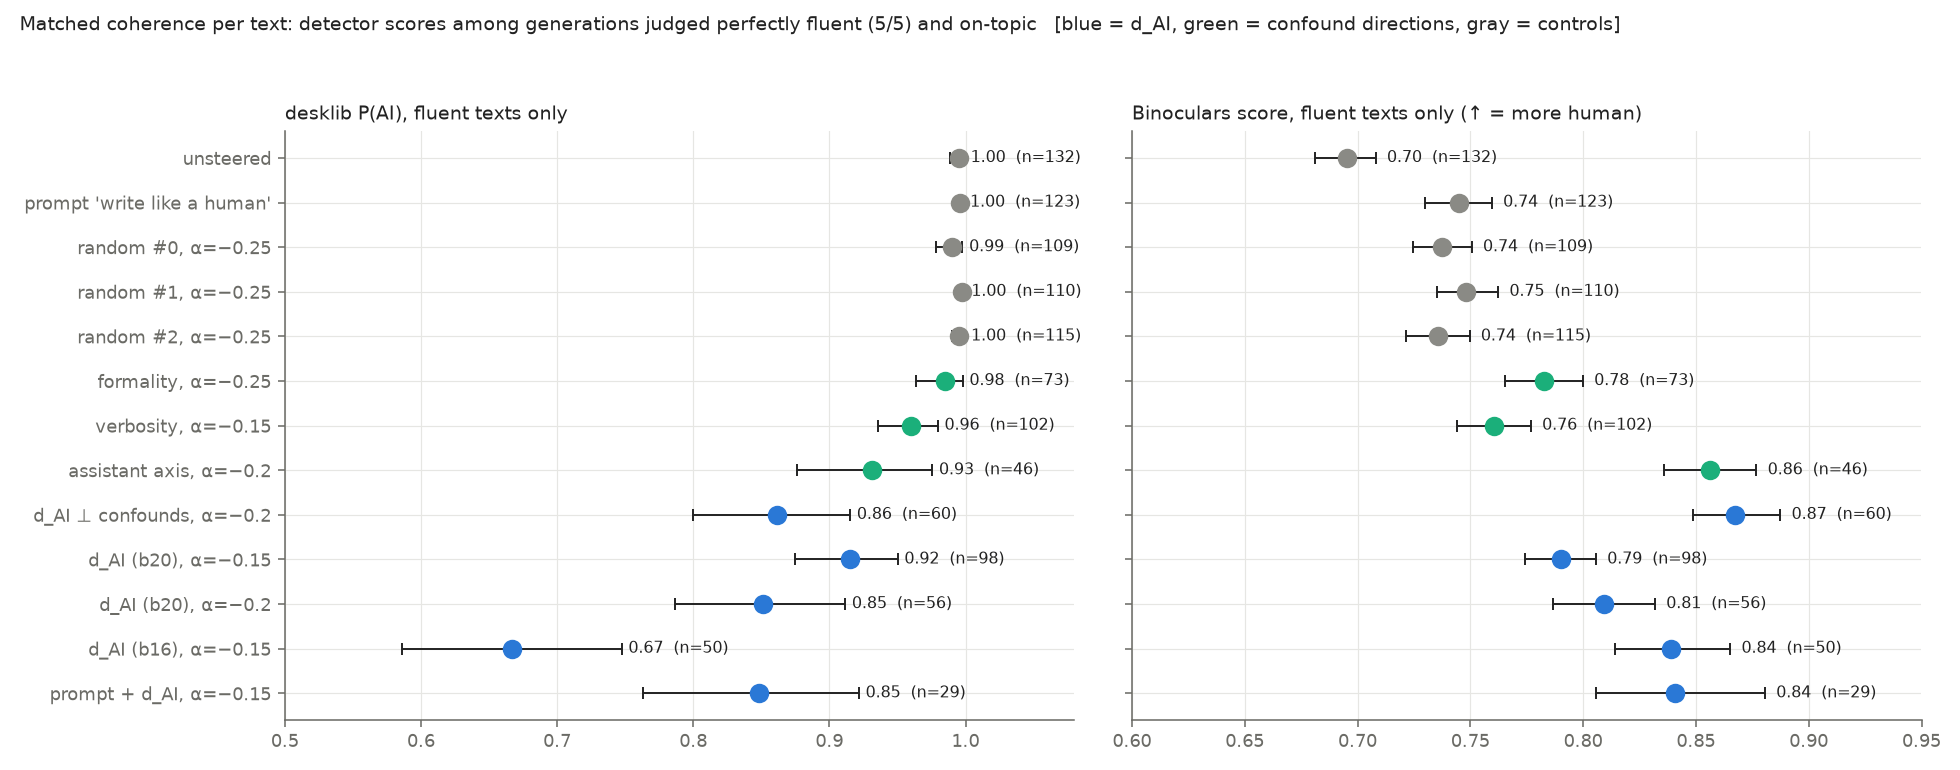
\includegraphics[width=0.99\linewidth]{figures/fig2_matched_coherence.png}
    \caption{Matched coherence per text. We keep only generations judged perfectly fluent (5/5), on-topic (relevance $\ge 4$), and in English. Among these, \dai and \daiperp (blue) still lower \desklib to 0.85--0.86 (0.67 at block 16), while random directions, the prompt (gray), and formality and verbosity (green) stay at 0.96--1.00. Error bars are 95\% bootstrap CIs; $n$ is the number of surviving texts.}
    \label{fig:matched}
\end{figure}

{\bf Is the effect just broken text?} No. \Figref{fig:matched} keeps only generations judged perfectly fluent and on-topic. In that subset, \dai at $\alpha=-0.2$ gives \desklib 0.85 ($n=56$) and \daiperp gives 0.86. Block-16 \dai gives 0.67, with 30\% of these fluent texts classified as human. By contrast, random directions give 0.99--1.00, formality 0.98, verbosity 0.96, the Assistant axis 0.93, and the prompt 1.00.
All \dai conditions differ from unsteered at $p<10^{-4}$ (Mann-Whitney); two of the three random directions do not differ significantly.
Per-condition matching agrees. We take the strongest $\alpha$ whose mean fluency and relevance stay within 0.5 of unsteered. \desklib is then 0.86 for \daiperp, 0.92 for \dai, 0.97 for the Assistant axis, 0.98 for formality, 0.99 for random, and 0.996 for the prompt.

{\bf Is \dai the Assistant persona?} No. Steering away from the Assistant axis lowers the detectors only once the text collapses: at $\alpha=-0.3$, \desklib is 0.78, but fluency is 1.34, relevance 1.02, and similarity to the unsteered answer 0.40. \dai moves the detectors while the answer and the assistant role stay intact.

\para{Binoculars is perplexity-confounded.} \binoculars rises under every perturbation, including random directions ($+0.09$ at $\alpha=-0.3$). Even among fluent texts, random steering moves it from 0.70 to 0.74, against 0.81 for \dai. The supervised detectors do not move under random steering, so we rely on them for the specificity claim.

\para{Positive steering.} Adding \dai cannot raise the supervised detectors, which are already at 0.996. It does raise the read-back projection to the ChatGPT-reference level (54.9 $\to$ 58.4) and, at $\alpha=+0.1$, lowers \binoculars to a more machine-like 0.68 ($p=0.001$). The base model, which is not at ceiling, shows the positive direction clearly (\secref{sec:base}).

\para{What changes in the text.} For the same prompt and seed, the unsteered answer opens ``{\em The forms 1099-MISC and K-1 serve different purposes in the tax system\ldots\ Let's break down each form: 1.\ **1099-MISC**: \ldots}''. At $\alpha=-0.25$ it becomes ``{\em I think you are mixing up two different things in taxation here: 1099-MISC and K-1. They are not to do with duplicate numbers, but are two differents tax forms\ldots}''.
Steering toward human adds first-person hedging, informal abbreviations, and small errors, while the answer keeps its topic and structure. Part of what detectors read as ``human'' is therefore {\em less polish}.

\para{Manipulation check.} At $\alpha=-0.25$, the unsteered model reads steered outputs exactly at the human level on \dai (read-back 35.8, equal to real human answers). Yet \desklib still gives 0.85, against 0.35 for human answers. Moving the model's own \dai coordinate to the human level captures only part of what external detectors respond to.

\subsection{In-distribution clamping: real but small}
\label{sec:clamp}

\begin{table}[t]
    \centering
    \resizebox{\textwidth}{!}{%
    \begin{tabular}{@{}lccccc@{}}
        \toprule
        Condition & \desklib & \fakespot & \binoculars & Fluency & Relevance \\
        \midrule
        \multicolumn{6}{@{}l}{\em Base model \qwenbase (Q/A completion format)} \\
        Unsteered & 0.938 & 0.772 & 0.740 & 4.66 & 4.18 \\
        Own \daibase $\alpha=-0.2$ & {\bf 0.870} & 0.693 & {\bf 0.818} & 4.31 & 3.63 \\
        Own \daibase $\alpha=+0.3$ & 0.959 & {\bf 0.914} & {\bf 0.670} & 4.69 & 4.49 \\
        Instruct \daiinst $\alpha=-0.2$ / $+0.3$ & 0.870 / 0.957 & 0.699 / 0.916 & 0.817 / 0.667 & 4.35 / 4.70 & 3.59 / 4.57 \\
        Random $\alpha=-0.2$ / $+0.3$ & 0.940 / 0.903 & 0.792 / 0.786 & 0.759 / 0.745 & 4.68 / 4.62 & 4.19 / 4.05 \\
        \midrule
        \multicolumn{6}{@{}l}{\em Instruct model \qwen, mean-clamp of the \dai coordinate} \\
        Unsteered & 0.996 & -- & 0.700 & 4.88 & -- \\
        Clamp b20 $\to$ AI mean & 0.997 & -- & 0.701 & 4.89 & -- \\
        Clamp b20 $\to$ human mean & 0.988 & -- & 0.727 & 4.89 & -- \\
        Clamp b20 $\to$ human mean $-$ 1 s.d. & {\bf 0.960} & -- & {\bf 0.757} & 4.82 & -- \\
        Clamp b10--27 $\to$ human mean & 0.967 & -- & 0.749 & 4.79 & -- \\
        Random directions, same clamp (3) & 0.994--0.996 & -- & 0.698--0.704 & 4.91--4.93 & -- \\
        \bottomrule
    \end{tabular}
    }
    \caption{{\em Top:} in the base model, \dai is causal in both directions, and the instruct model's direction works identically; random directions have no significant effect. Bold marks the strongest effect in each direction. {\em Bottom:} in-distribution clamping of the \dai coordinate in the instruct model gives small but direction-specific shifts with no fluency cost.}
    \label{tab:base_clamp}
\end{table}


Zero-ablating \dai destroys the text (fluency 1.00), because the human mean projection is not zero (32 at block 20). We therefore clamp the coordinate within its natural range instead (\tabref{tab:base_clamp}, bottom; \figref{fig:base}, right).
Clamping to the AI mean does nothing, since generations already sit there (54.9 \versus 53.6), which serves as a consistency check. Clamping to the human mean minus one standard deviation lowers \desklib to 0.960 and raises \binoculars to 0.757, with no fluency cost. Against the same clamp on random directions, the differences are $-0.034$ [$-0.052$, $-0.020$] for \desklib and $+0.057$ for \binoculars (both $p_{\text{holm}}<10^{-4}$).
The effect is specific but small. For scale, additive steering at $\alpha=-0.2$ shifts the coordinate by 71 units, about $3.3\times$ the natural human--AI gap of 21 units. Large detector effects need extrapolation beyond the range that human text occupies.

\subsection{Base \versus instruct: present before chat tuning (H4)}
\label{sec:base}

\begin{figure}[t]
    \centering
    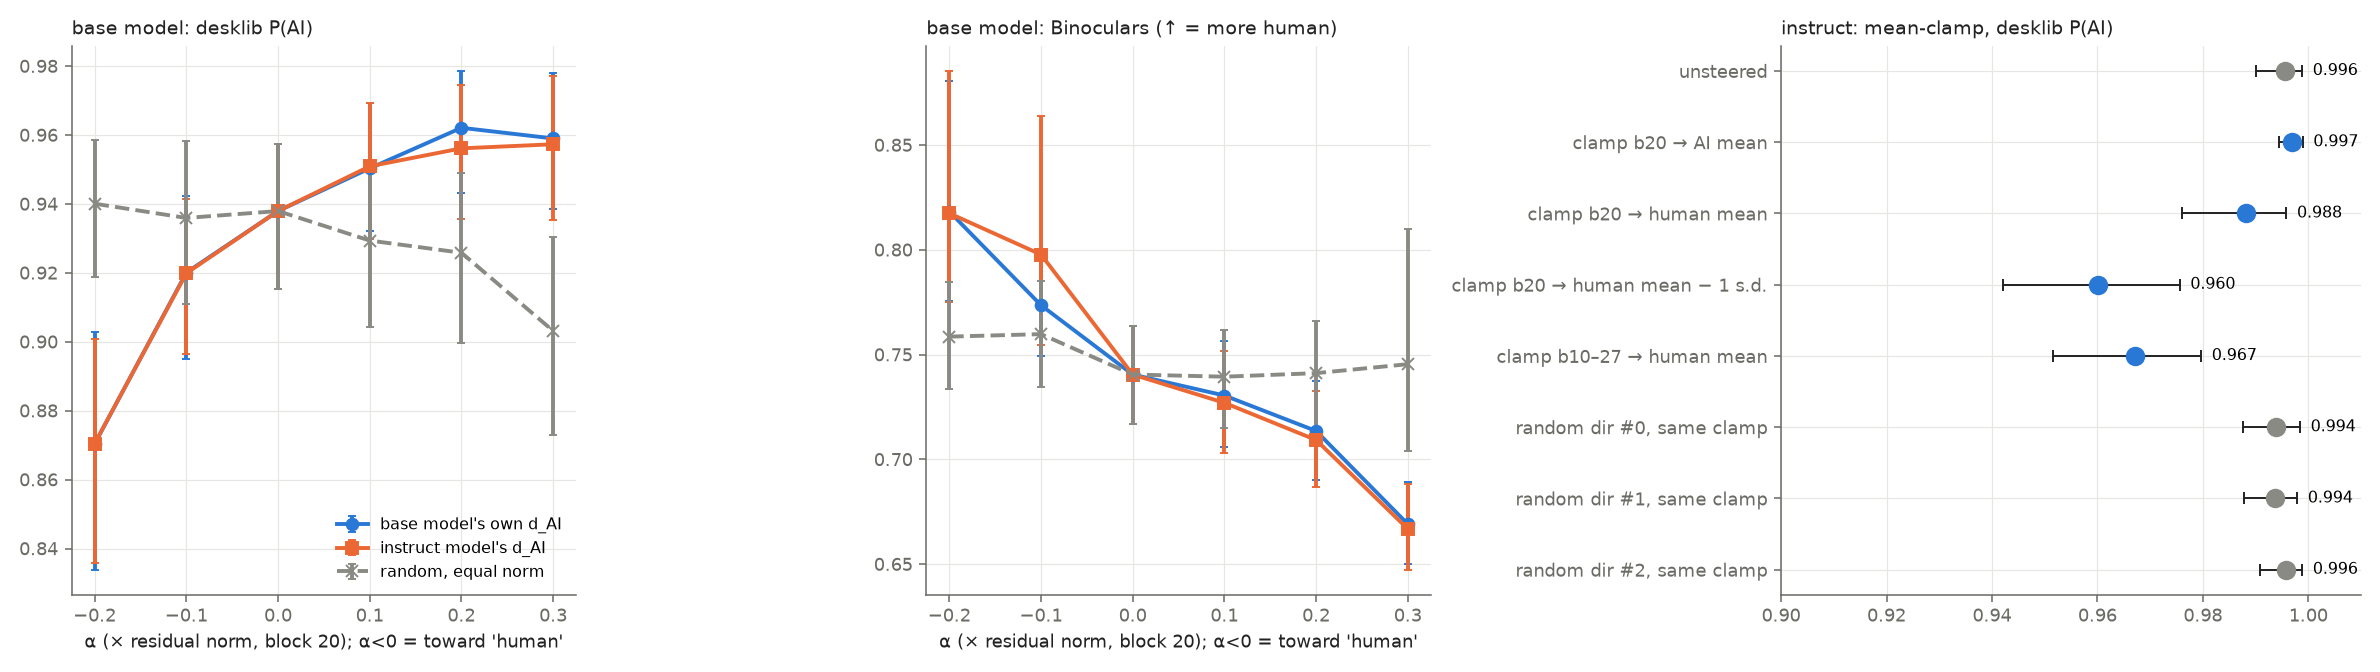
\includegraphics[width=0.99\linewidth]{figures/fig3_base_and_clamp.png}
    \caption{\figleft{} and \figcenter{} Steering the base model \qwenbase. Its own \dai (blue) and the instruct model's \dai (orange) give identical, bidirectional effects on \desklib and \binoculars, while a random direction (gray) is flat. \figright{} In-distribution mean-clamp in the instruct model. Clamping the \dai coordinate toward the human range gives small but direction-specific drops in \desklib; the same clamp on random directions has no effect.}
    \label{fig:base}
\end{figure}

The base and instruct directions are nearly identical: $\cos(\daibase,\daiinst)$ ranges from 0.984 to 0.995 across layers (0.991 at block 20). Base-model read-out is as good or slightly better (\tabref{tab:readout}; Cohen's $d$ 1.20 \versus 1.00 at block 20). Chat tuning neither creates nor sharpens the read-out direction.

In the base model, steering works in {\em both} directions (\tabref{tab:base_clamp}, top; \figref{fig:base}). Subtracting \daibase at $\alpha=-0.2$ lowers \desklib from 0.938 to 0.870 ($p_{\text{holm}}=8\times10^{-4}$) and raises \binoculars to 0.818. Adding it at $\alpha=+0.3$ raises \fakespot from 0.77 to 0.91 and lowers \binoculars to 0.670, while slightly {\em raising} relevance (4.18 $\to$ 4.49) and lengthening answers from 81 to 99 words. The instruct model's direction has the same effect, and random directions have no significant effect.
Base \qwenbase answers already look AI-like (\desklib 0.94; read-back 57.7, close to the ChatGPT references), consistent with a pretraining corpus that contains much synthetic and instruction-style data. Chat tuning moves the model's outputs further along the direction (\desklib 0.94 $\to$ 0.996, $p<10^{-4}$) without changing the direction itself.

\subsection{LLM judges: same sign, different ranking}
\label{sec:judges}

\begin{table}[t]
    \centering
    \resizebox{\textwidth}{!}{%
    \begin{tabular}{@{}lccccc@{}}
        \toprule
        Condition & AI-likelihood & $\Delta$ \versus unsteered [95\% CI] & $p_{\text{holm}}$ & Fluency & \% rated $<50$ \\
        \midrule
        Unsteered & 73.9 & -- & -- & 4.26 & 2\% \\
        \dai $\alpha=-0.15$ & 67.4 & $-6.2$ [$-10.7$, $-2.1$] & 0.038 & 4.06 & 8\% \\
        \dai $\alpha=-0.2$ & 67.7 & $-6.2$ [$-9.6$, $-3.0$] & 0.038 & 3.56 & 4\% \\
        \dai $\alpha=-0.25$ & 63.0 & $-10.9$ [$-17.5$, $-4.7$] & 0.061 & 2.64 & 20\% \\
        \daiperp $\alpha=-0.2$ & 68.5 & $-5.4$ [$-9.3$, $-1.9$] & 0.092 & 3.88 & 6\% \\
        Formality $\alpha=-0.25$ & 65.6 & {\bf $-$8.3} [$-11.7$, $-4.9$] & 0.001 & 3.70 & 8\% \\
        Assistant axis $\alpha=-0.2$ & 71.9 & $-2.0$ & 1.0 & 3.32 & 6\% \\
        Random 0/1/2 $\alpha=-0.2$ & 73.2/70.4/71.7 & $-0.7$/$-3.5$/$-2.2$ & $\ge 0.37$ & 4.18--4.20 & 0--2\% \\
        Prompt ``write like a human'' & 67.2 & $-6.7$ [$-9.8$, $-3.6$] & 0.004 & {\bf 4.24} & 6\% \\
        \dai $\alpha=+0.2$ & 75.3 & $+1.4$ & 1.0 & 3.94 & 0\% \\
        \midrule
        {\em \hcthree human answers} & {\em 54.5} & & & {\em 3.58} & {\em 38\%} \\
        {\em \hcthree ChatGPT answers} & {\em 69.8} & & & {\em 4.04} & {\em 0\%} \\
        \bottomrule
    \end{tabular}
    }
    \caption{Blind Cohere command-a-plus judge (0--100 AI-likelihood; 50 prompts per condition; Holm over 22 tests). The judge sees \dai lower AI-likelihood more than random directions do, but formality steering and prompting do at least as well. The judge itself is only weakly valid (AUROC 0.71).}
    \label{tab:cohere}
\end{table}


The blind Cohere judge agrees on the sign (\tabref{tab:cohere}). \dai at $\alpha=-0.2$ lowers AI-likelihood by 6.2 points relative to unsteered, and by 4.1 [$-7.0$, $-1.0$] relative to the mean of the random directions ($p=0.005$). A partial Nemotron-3-Super run at $\alpha=-0.1$ ($n\approx150$ per condition) agrees: \dai minus random is $-4.0$ [$-7.2$, $-0.9$] ($p=0.03$).
On these judges, however, \dai is {\em not} specific. Formality steering ($-8.3$) and the ``write like a human'' prompt ($-6.7$, with no fluency cost) do as well or better. On Nemotron, formality, the Assistant axis, and \daiperp score 69.6--69.9, similar to \dai's 70.1.
The judges appear to respond to surface register (informality, contractions, no markdown), which formality steering and prompting change directly. The supervised detectors rank the methods the other way round: \dai is far ahead, and formality, prompting, and random are similar. This is a real split between measures, not noise. Different readers of ``AI-ness'' key on different features, and \dai targets the one the trained detectors use.
